\subsection{Facilities Evolution}
\label{Sec:FacilitiesFuture}

Planning is well underway to address the compelling physics questions presented in Section~\ref{Sec:Progress}. 
The evolution of the RHIC and LHC accelerators, accompanied by upgrades to their experiments, will provide tools uniquely suited
for determining the inner workings of thermal QCD matter. The prospect of these two facilities, operating with increased luminosity
and a range of energies spanning three orders of magnitude, coupled with greatly upgraded detector capabilities, provides an unprecedented
opportunity to resolve fundamental aspects of QCD.

\begin{figure}[ht]
\centerline{
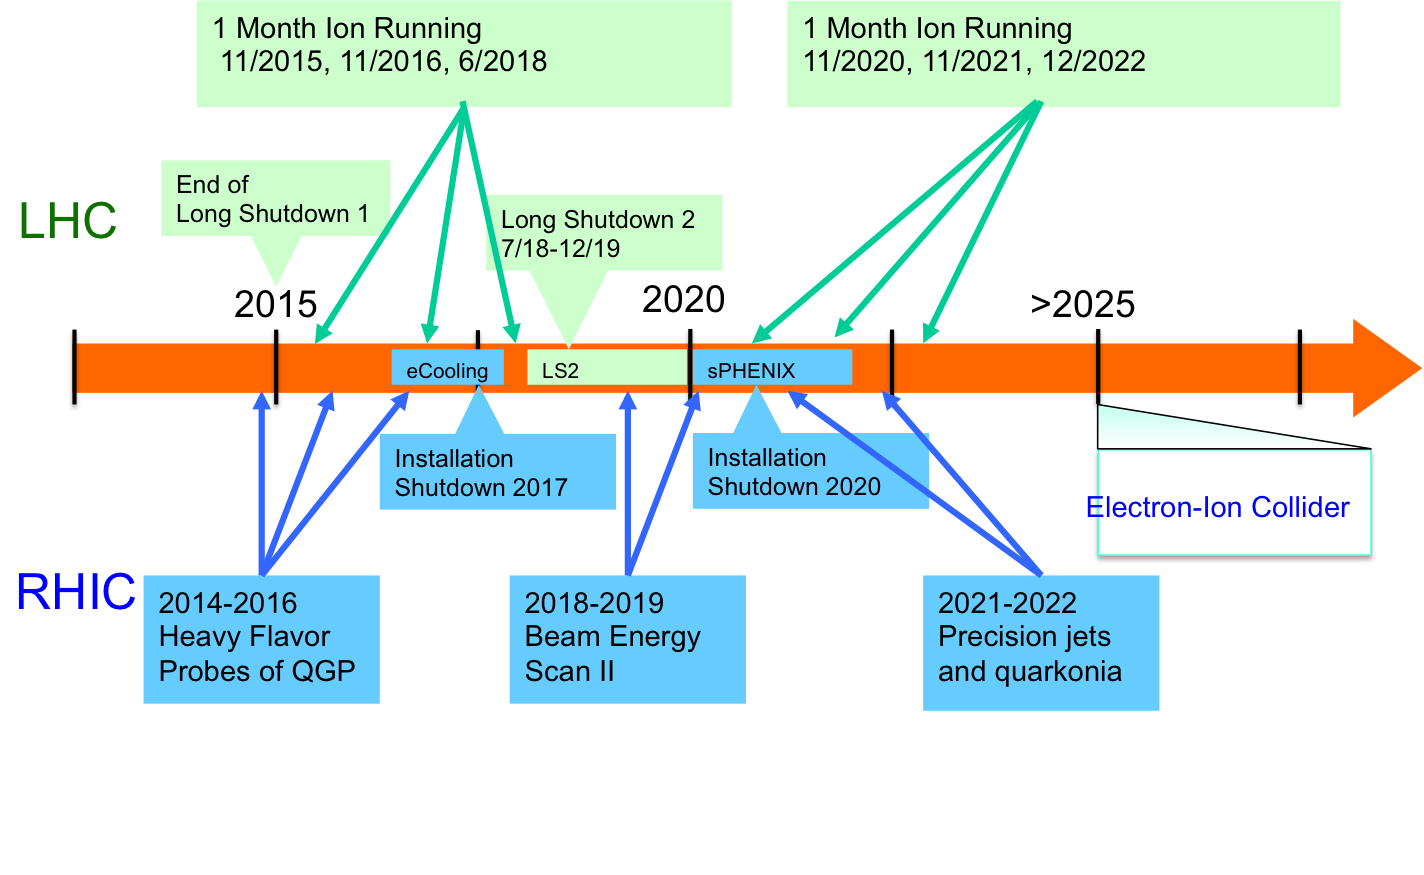
\includegraphics[width=1.00\textwidth]{fig/Timeline.png}
}
\caption{The timeline for future RHIC and LHC heavy ion running.
}
\label{Fig:Timeline}
\end{figure}

\subsubsection{Facility and experiment upgrades at RHIC}
\label{Sec:RHICUpgrades}
At Brookhaven National Laboratory, the goal for the next decade is to complete the  science mission of RHIC on a schedule that permits a smooth and timely transition towards preparations for an electron-ion collider based on the RHIC complex. 
A coherent physics program has been developed to address the outstanding questions in both hot and cold QCD physics 
relevant to completing our understanding of the QGP, with a natural physical and intellectual evolution towards the 
physics addressed by an electron-ion collider.
Accordingly, future heavy ion running is divided into three campaigns: 

\begin{itemize}[leftmargin=2.0cm]

\item[\bf 2014-16:] Measure heavy flavor probes of the QGP using the newly installed silicon vertexing detectors in PHENIX and STAR.
\item[\bf 2018-19:] Conduct a fine-grained scan of the QCD phase diagram via Phase II of the RHIC Beam Energy Scan program.
\item[\bf 2021-22:] Perform precision jet quenching and quarkonia measurements following the installation of sPHENIX.

\end{itemize}

Interspersed between these three running periods are two shutdowns, as illustrated in Figure~\ref{Fig:Timeline}. 
\begin{figure}[!htp]
\centerline{
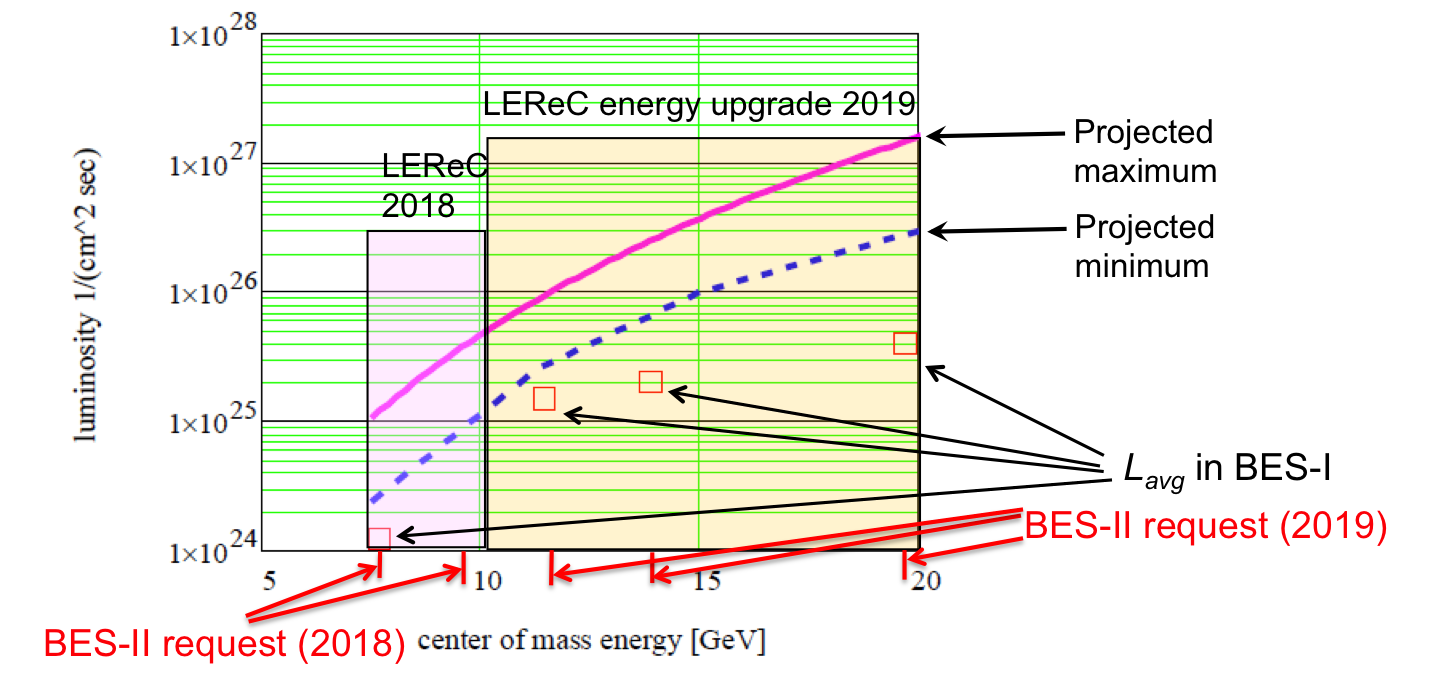
\includegraphics[width=1.00\textwidth]{fig/RHICeCooling.png}
}
\caption[Projected RHIC luminosity increase at low energies from electron cooling]{The projected RHIC luminosity increase at low energies provided by electron cooling of the ion beams. The red squares are the measured average luminosity in RHIC Beam Energy Scan~I. The blue dashed line is the minimum projection for the improvement with electron cooling; the magenta solid line is the maximum projection. Also shown are the actual luminosities achieved in RHIC BES~I. 
}
\label{Fig:eCooling}
\end{figure}
The first shutdown, in 2017,  is to allow for installation of electron cooling to increase RHIC's luminosity
at low energies\footnote{It should be noted that the current RHIC performance at low energies exceeds the original design values for luminosity by well over an order-of-magnitude. In fact, the original RHIC design was limited to energies of 20 GeV and above.}, 
as shown in Figure~\ref{Fig:eCooling}. This luminosity upgrade, in combination with targeted upgrades of the STAR detector described below, greatly increases the discovery potential of the subsequent beam energy scan in 2018-2019. The second shutdown, in 2020, will be used to install the sPHENIX detector (discussed below), prior to a period of dedicated running to explore the microscopic structure of the QGP with high energy jets and quarkonia measurements. Both the sPHENIX upgrade and the proposed STAR upgrades provide natural evolution paths towards detectors for the EIC\footnote{In addition to the upgrade paths from sPHENIX to ePHENIX and STAR to eSTAR, consideration has been given
to a new detector explicitly designed for electron-ion capabilities. Details are available in Refs.~\cite{Accardi:2012qut,Boer:2011fh}
}.

\begin{figure}[!htp]
   \centering
       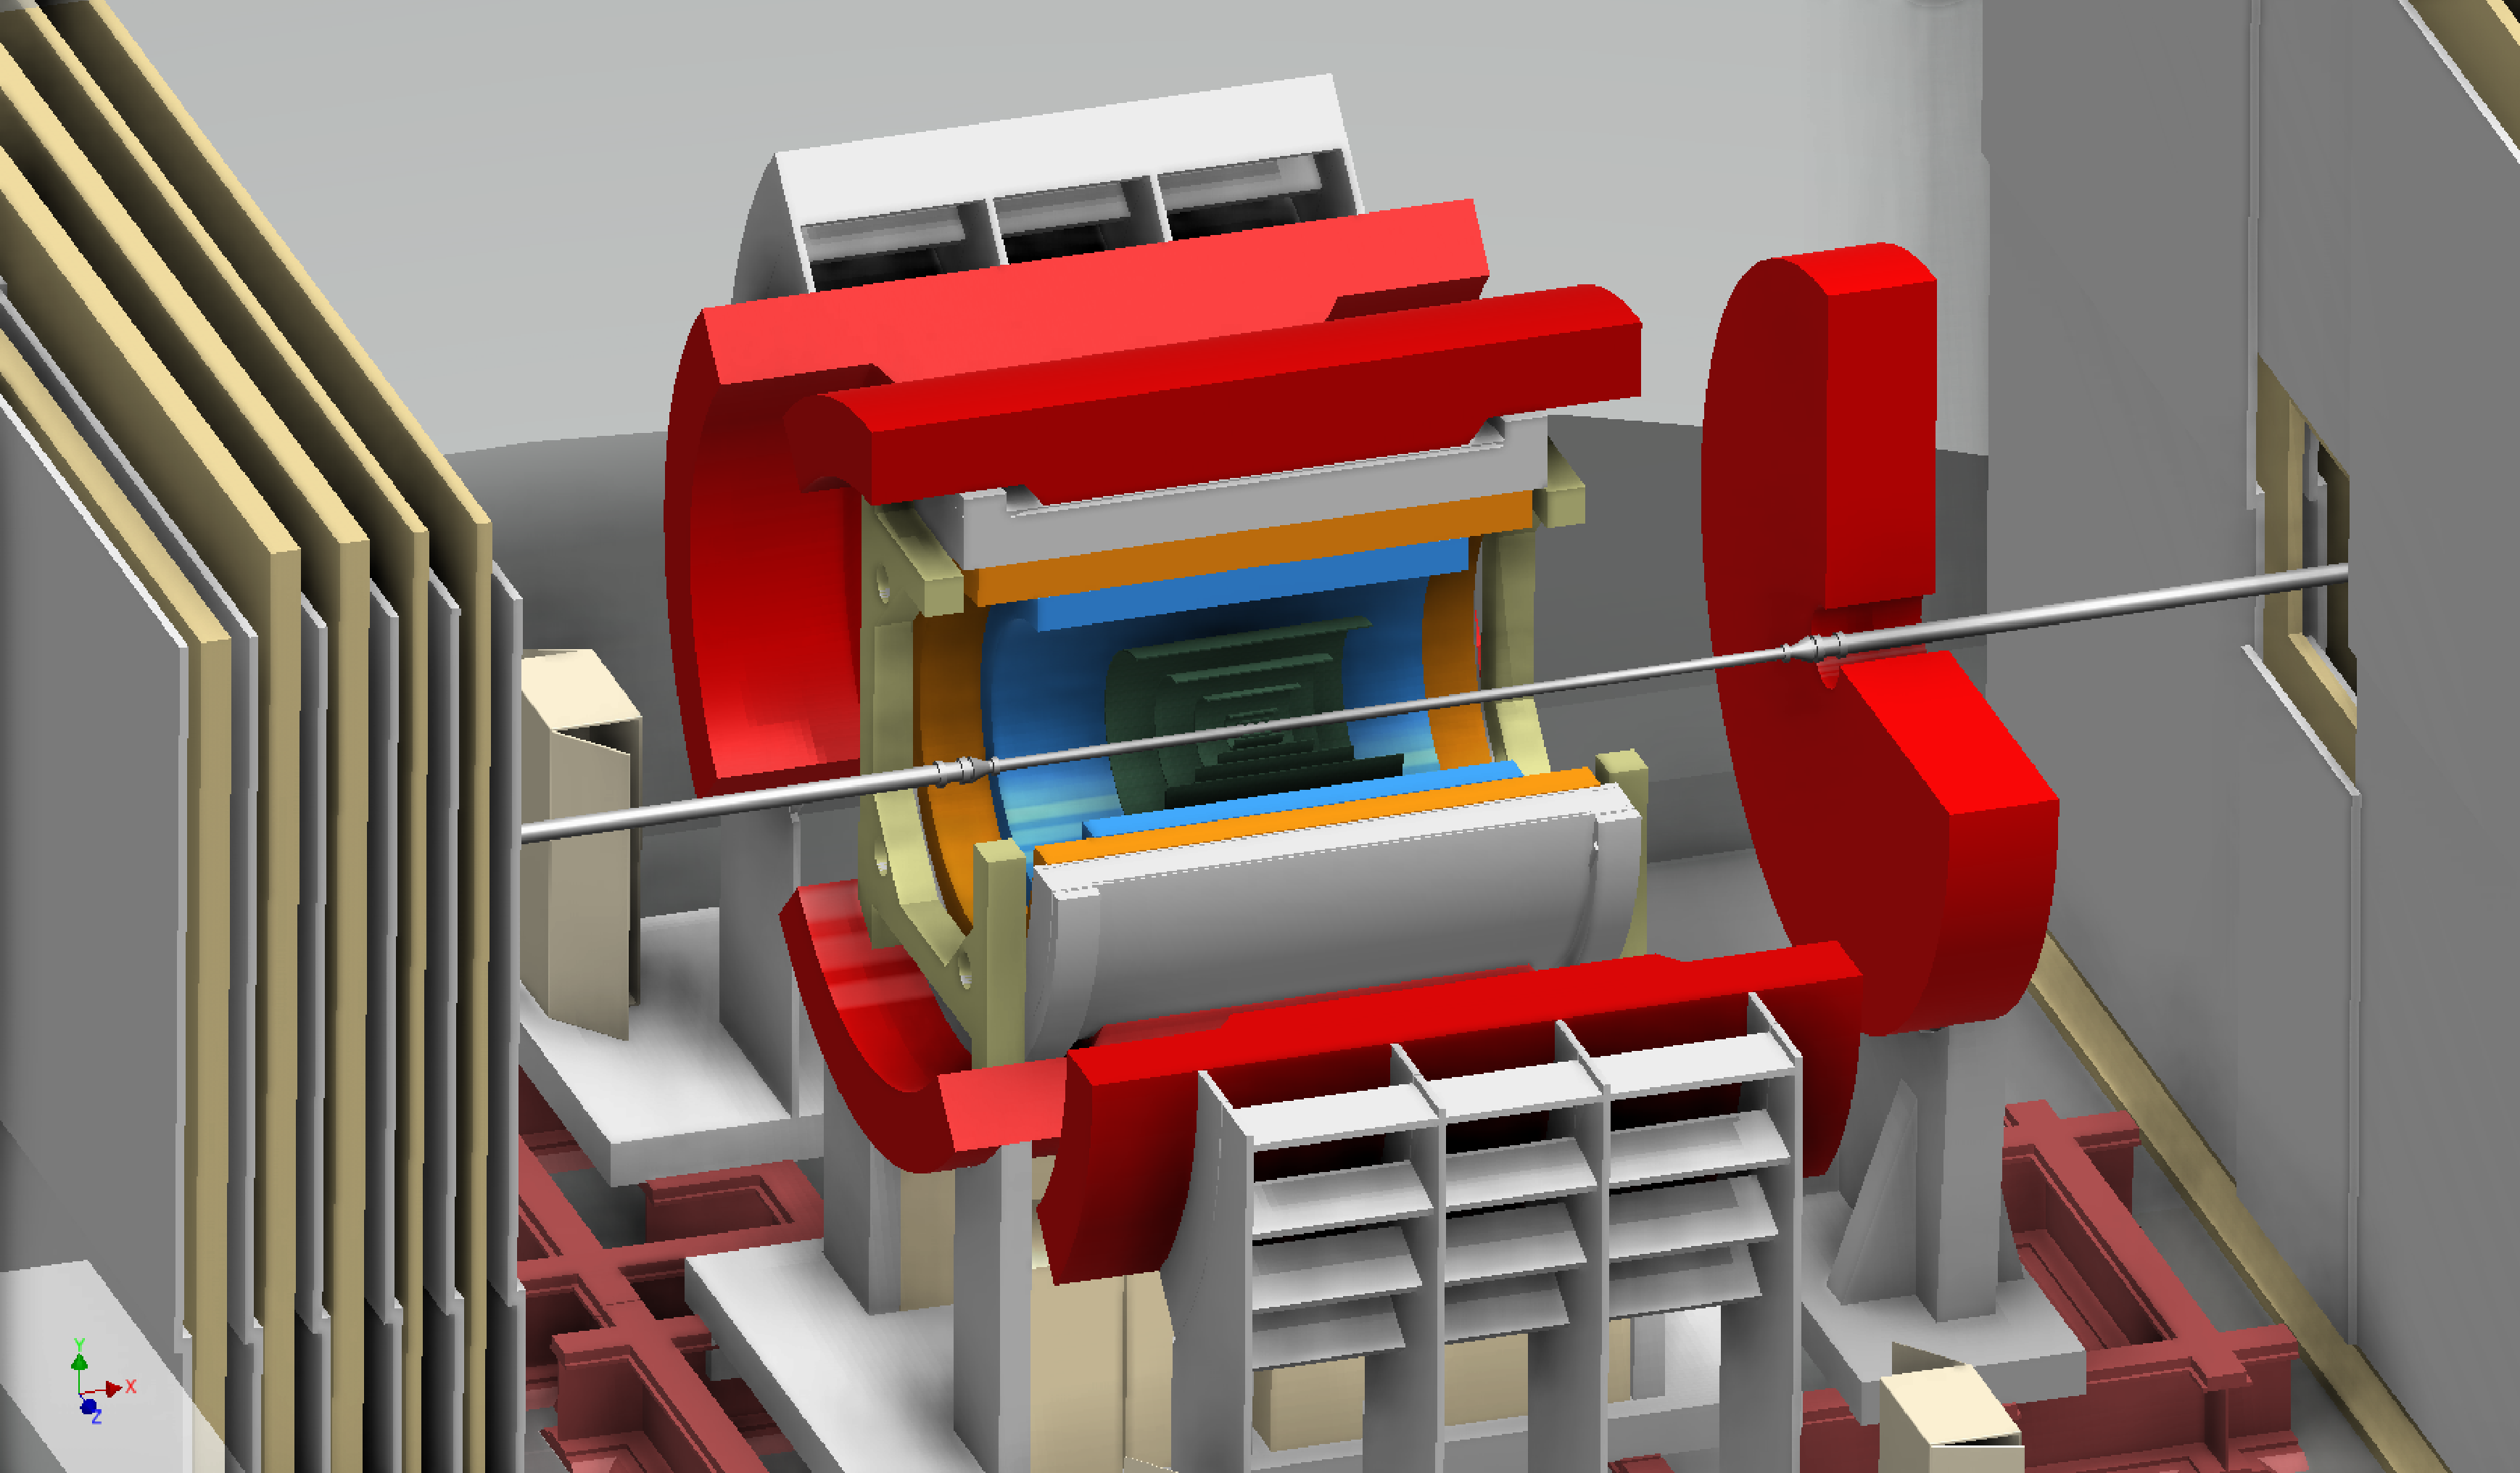
\includegraphics[width=0.9\linewidth]{fig/sPhenix-3D-Hall-Cutout.pdf}
       \vskip 4mm
       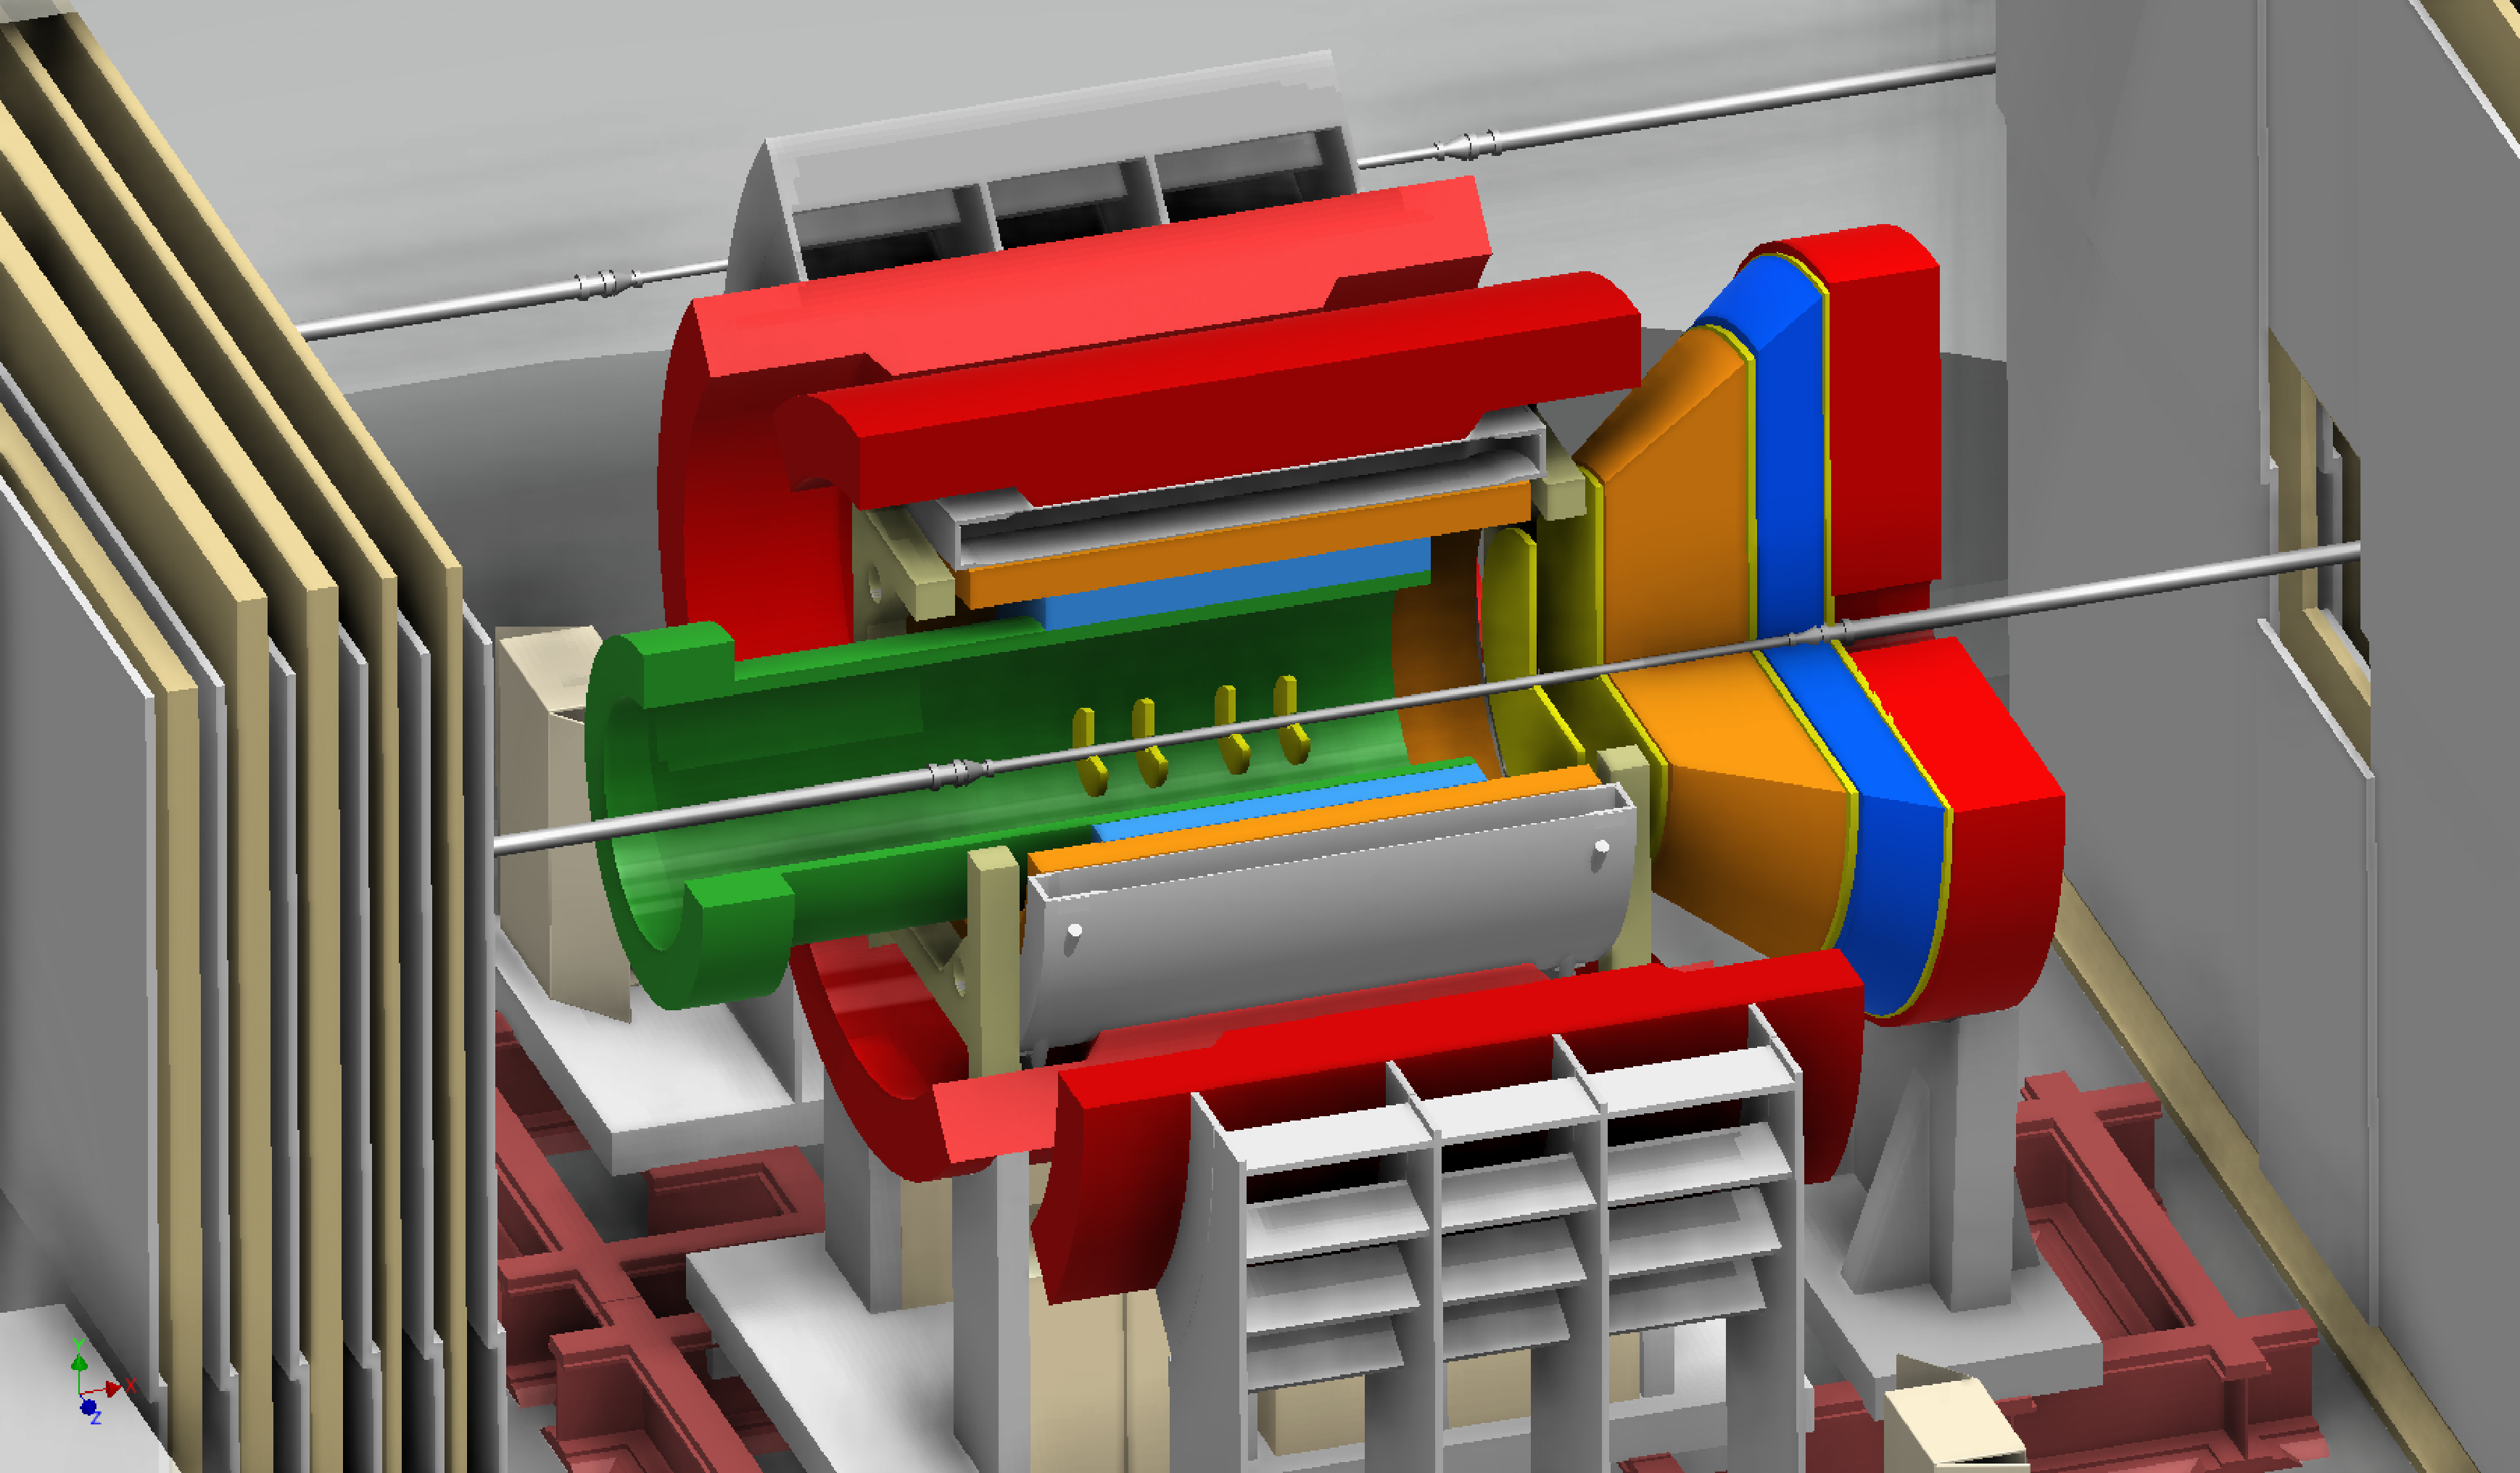
\includegraphics[width=0.9\textwidth]{fig/ePhenix-Cut-Out-View.pdf}
       \caption[Proposed sPHENIX upgrade and its evolution to an EIC detector]{ (top) An engineering rendering of the proposed
         sPHENIX upgrade to the PHENIX experiment, showing the inner
         tracking system, the electromagnetic calorimeter, the BaBar
         solenoid and the hadronic calorimeter. (bottom) The evolution
         of the sPHENIX detector into a full-capability EIC detector.}
       \label{Fig:sPHENIX}
       \label{Fig:ePHENIX}
\end{figure}

{\bf sPHENIX:} The PHENIX collaboration has submitted a
proposal\cite{Aidala:2012nz} to the DOE for MIE funding (Major Item of
Equipment) to replace the PHENIX central detectors in order to provide
full hadronic and electromagnetic calorimetry along with charged
particle tracking over a pseudorapidity interval $\eta < 1$ The new
apparatus, sPHENIX, shown in Figure~\ref{Fig:sPHENIX} would
dramatically extend the range of jets measurable at RHIC and provide
precision spectroscopy of quarkonia.  With a mass resolution of better
than 100~MeV/$c^2$, sPHENIX will separately measure the $1S$, $2S$ and
$3S$ states of the upsilon, providing key information about Debye
screening in the QGP.  The full sPHENIX physics program employs
inclusive jet, dijet, $b$-tagged jet, $\gamma$$+$jet, high transverse
momentum charged hadron, jet fragmentation function, and upsilon
measurements to enable a very comprehensive and detailed investigation
of the microscopic dynamics of the QGP in the temperature range where
its coupling is at its strongest.

The very high data acquisition bandwidth of sPHENIX, combined with
RHIC~II luminosities, brings fundamentally new capabilities to the
measurement of hard probes at RHIC.  In one year, sPHENIX will record
100 billion minimum bias Au$+$Au collisions, providing an extremely
large sample of unbiased jets.  This enormous sample will be further
augmented by calorimetric triggers sampling more than 2/3 of a
trillion top-energy Au$+$Au collisions made possible by the RHIC~II
luminosity.  All told, this enables the measurements of jets in
$p$$+$$p$, $p$$+$Au and Au$+$Au beyond 70~GeV and a correspondingly
large kinematic reach for other hard probes, as shown in
Figure~\ref{fig:AAphysics_projections}.

\begin{figure}[hbt!]
  \centering
  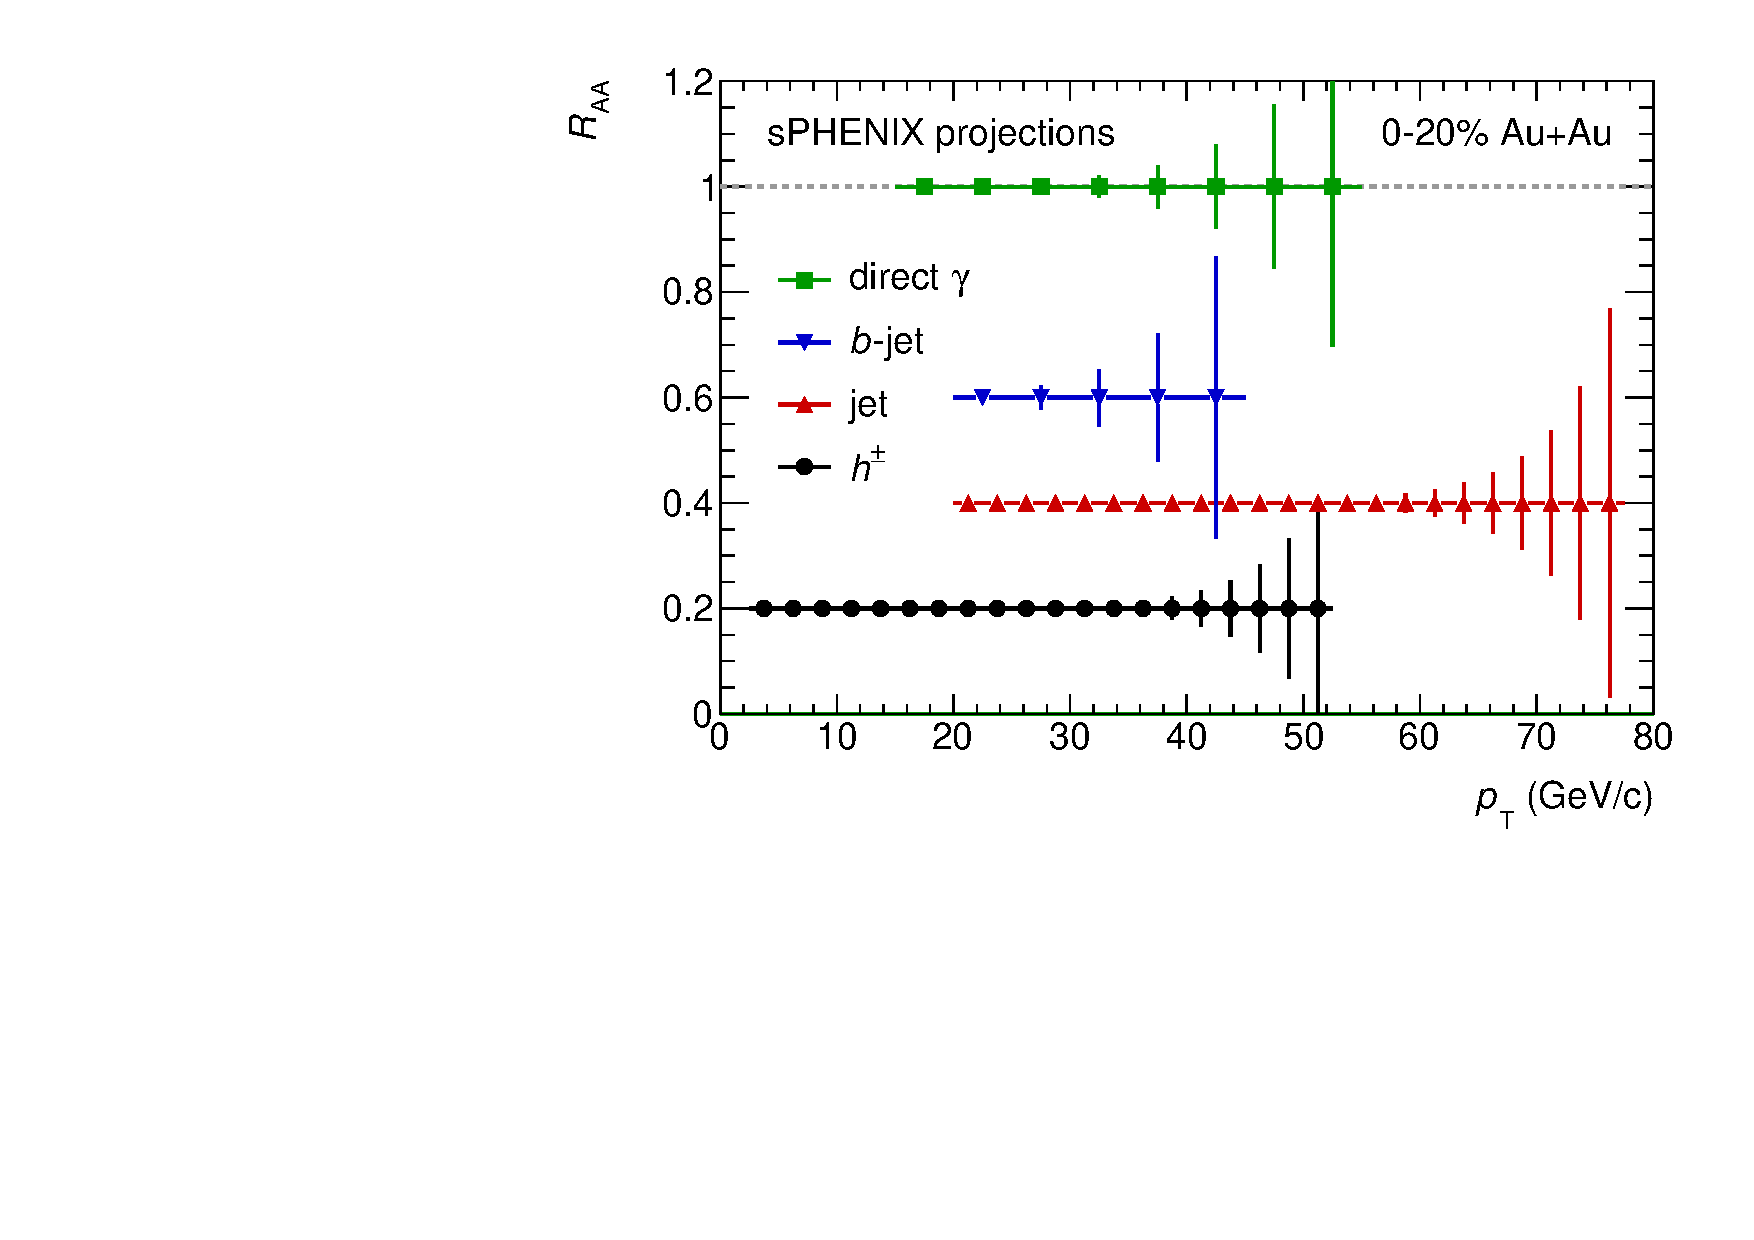
\includegraphics[width=0.8\textwidth]{fig/sPHENIX_MIE_master_AuAu_projections}
  \caption[Projected sPHENIX statistical uncertainties on $R_\mathrm{AA}$
    for $\gamma$'s, jets, $b$-jets and $h^\pm$]{Projected statistical uncertainties on the $R_\mathrm{AA}$
    for inclusive photons (green points, assuming $R_\mathrm{AA} =
    1$), $b$-jets (blue points, assuming $R_\mathrm{AA} = 0.6$),
    inclusive jets (red points, assuming $R_\mathrm{AA} = 0.4$) and
    charged hadrons (black points, assuming $R_\mathrm{AA} =
    0.2$). These projections are made with a $b$-jet tagging
   efficiency of $50$\%, 10 weeks of $p$+$p$ and 22 weeks of Au$+$Au
    data taking.}
    \label{fig:AAphysics_projections}
\end{figure}

This reach in $Q^2$, combined
with precision vertexing provides the basis for a compelling program of direct comparisons to corresponding measurements at the LHC
discussed in Sections~\ref{Sec:FutureJetCapabilities}, \ref{Sec:FutureJetProbes} and \ref{Sec:FutureQuarkonia}. The sPHENIX design takes advantage of recent technological advances in sensors and read-out electronics to minimize costs. In addition, the superconducting solenoid from the BaBar experiment at SLAC has been transferred to BNL\cite{BabarMove} for use in sPHENIX, resulting in a very considerable cost savings. Finally, the sPHENIX design provides a route for a smooth evolution to a full-capability EIC detector\cite{Adare:2014aaa}, shown in Figure~\ref{Fig:ePHENIX}. In addition, there is a an exciting extended program of polarized p+p and p+A\cite{PHENIXpppA,Aschenauer:2015eha}
if some of the EIC detector can be realized earlier.

{\bf STAR Upgrades:} The STAR experiment has recently installed two new detector sub-systems: the Heavy Flavor Tracker discussed in Sections~\ref{Sec:Facilities} and Section~\ref{Sec:OpenHF}, and the Muon Telescope Detector described in Section~\ref{Sec:Quarkonia}.
With the completion of the HFT and the MTD,
STAR's upgrade plans next focus on  Phase II of the RHIC Bean Energy Scan.  The inner sectors of the TPC will be replaced to allow full coverage of pads increasing the pseudorapidity coverage, and extending momentum coverage to lower \pT\ . In addition STAR will  add an event plane detector which will enrich the STAR BES program by allowing for an independent measurement of the event plane  and significantly improving its resolution .  Both these and longer term upgrades improve STAR's forward capabilities 
in preparation for an eSTAR configuration in the EIC era\cite{STAR:eSTAR} as outlined in Figure~\ref{Fig:STARplan}.  
\begin{figure}[!htp]
\includegraphics*[width=0.9\textwidth]{fig/starplan_jan2015.pdf}
\vspace{-0.5cm}
\caption[STAR upgrade plan towards an EIC detector]{The STAR upgrade plan,
showing the evolution from the current configuration focused on \pp\ and \AplusA\ physics at
mid-rapidity to a design emphasizing forward physics in \pp\ and \pA\ collisions\cite{STAR:FU,STAR:DecadalPlan}
and later  $e$+p and $e$+A physics at an EIC~\cite{STAR:eSTAR}.}
\label{Fig:STARplan}
\end{figure}

The STAR near-term proposed upgrades relevant to BES-II include:
\begin{itemize}
\item[] {\bf iTPC upgrade:} The STAR collaboration has proposed to upgrade the inner sectors of the read-out plane of the Time-Projection-Chamber (iTPC)~\cite{STAR:BESII}  in order to increase the segmentation on the inner pad plane and to renew the inner-sector wires. This upgrade will improve the resolution on both momentum and $dE/dx$ resolution, increase the track reconstruction efficiency and extend the  acceptance in 
pseudorapidity  from $|\eta| \le 1.1$ to $|\eta| \le 1.7$.
%Although iTPC will allow significantly improved tracking and coverage out to $|\eta| \le$ 1.7, the longitudinal boost for higher rapidity particles shifts the low $p_T$ particles into a momentum range where it becomes increasingly challenging to employ PID through relative ionization in the TPC. 
The enhanced performance made possible by the iTPC will not only benefit the BES-II physics program but will also be crucial for STAR�s future program with \pp\ / \pA\ and $e$+p/$e$+A collisions at the forward high-rapidity regions.

\item[] {\bf EPD:} The proposed Event Plane Detector (EPD) is a dedicated event-plane and centrality detector placed in the forward rapidity region 2 $\le | \eta| \le$ 4. With segmentation in both radial and azimuthal directions, the detector will provide precise measurements of the collision centrality and the event plane, as well as serving as a trigger detector for collisions at lower beam energies.
%The proposed EPD configurations with 12 or 30 ?-segmentations are both very close to the optimal case. 
The EPD will be crucial for the physics measurements of collectivity as well as correlations in a much wider rapidity region. 
\end{itemize}

In the longer term STAR has proposed a series of mid-rapidity and forward upgrades that are complementary to the sPHENIX
physics program described above. The planned upgrades include:
\begin{itemize}
\item {\bf HFT$^+$:} The current HFT pixel integration time of $\sim 200~\mu$sec is much longer 
than the $\le 40~\mu$sec of the STAR TPC . 
In order to synchronize the TPC and HFT read-out for maximum rate capability for measuring bottom quark production at RHIC, the STAR collaboration has started design studies on the HFT$^+$, a faster version of the HFT with the state of art pixel technology. 
New technological developments permit read-out times less than
$20~\mu$sec without any increase of power consumption, so that the HFT support infrastructure
for cooling and power can be re-used for the HFT$^+$, making it a very cost-effective upgrade. 
%The HFT$^+$ allows tagging of bottom hadron productions at the top RHIC energies. 
The physics enabled by the HFT$^+$ physics is complementary to sPHENIX's jet program as well as ALICE's upgraded heavy flavor program
(to begin in 2019) at the LHC. In addition, the faster HFT$^+$ will be helpful for the heavy flavor physics in the spin program at RHIC.

{\bf Forward Upgrades:} The STAR collaboration has developed plans~\cite{STAR:FU,STAR:DecadalPlan} for measurements with forward photons, $J/\Psi$'s, Drell-Yan pairs, and di-jet and hadron/jet correlation probes, as well as $W$ and $Z$ bosons at top RHIC energy.
%and demonstrate measurement capability and sensitivity through detailed simulations. It will be shown that these probes allow addressing fundamental aspects of the nucleon partonic structure, which are still rather poorly determined by experiment. One is the nature of the nucleon spin; the other is go beyond our current simple one-dimensional picture of nucleons by correlating the information on the individual parton contribution to the spin of the nucleon with its transverse momentum and spatial distribution inside the nucleon. 
Measuring these probes in \pA\ collisions will further our understanding of cold nuclear matter effects in QCD processes in cold nuclear matter by studying the dynamics of partons at very small and very large momentum fractions $x$ in nuclei, and at high gluon density to investigate the existence of nonlinear evolution effects. STAR's forward upgrade plan is centered around the unique capabilities afforded with the existing STAR detector, complemented with detector upgrades including the forward calorimetric system (FCS) and forward tracking system (FTS), which are required to carry out the proposed physics program at forward rapidities. The proposed FCS and FTS upgrades were first envisioned in the STAR Decadal Plan~\cite{STAR:DecadalPlan} and represent a natural evolution of the growth of the STAR scientific program. These upgrades will be an integral part of the eSTAR configuration at eRHIC outlined in the eSTAR letter of intent~\cite{STAR:eSTAR}, see Figure~\ref{Fig:eSTAR}.
\begin{figure}[!htp]
\includegraphics*[width=0.9\textwidth]{fig/estar_proposal.pdf}
\vspace{-1.5cm}
\caption[eSTAR layout with proposed upgrades]{eSTAR layout with the proposed upgrades of the iTPC, Forward Calorimetry System (FCS), Forward Tracking System (FTS), Endcap TOF (E/W TOF), BSO Crystal Calorimeter (CEMC), and a GEM-based transition radiation detector. In this configuration, the electron beam is from right to left while hadron beam from left to right~\cite{STAR:eSTAR}. }
\label{Fig:eSTAR}
\end{figure}
\end{itemize}



\subsubsection{Facility and experiment upgrades at the LHC}

Following the successful Run I p+p, Pb+Pb and p+Pb data taking periods, the LHC is now preparing
for Run II, forseen to include p+p, p+Pb and heavy ion data taking from 2015 to 2018. Run II
will be followed by a shutdown from 2018 to 2020 (LS2) and Run III from 2020 to 2023.
For both the p+p and Pb+Pb data taking, the LHC upgrades during the current shutdown should
allow for collisions at close to the design energy, i.e., $\sim$5~TeV for Pb+Pb. In addition, a
large increase in the Pb+Pb instantaneous luminosity is projected, with collision rates expected
to exceed those achieved in Run I by up to one order of magnitude. Combining Run II and III,
the LHC goal is to deliver about 10~nb$^{-1}$  of Pb+Pb collisions to each of ALICE, ATLAS and CMS. In combination,
the increased collision energy and luminosity will increase statistics for rare high \pT\
probes by about a factor of 200.

To exploit the improved accelerator performance, ALICE, ATLAS and CMS are undergoing
significant upgrades during the current shutdown and in the future LS2. For ATLAS and CMS, these upgrades
are mostly driven by the needs of the p+p program. Further large luminosity increases for
\pp\ will produce a larger number of collisions per bunch crossing (``pileup''), eventually
reaching multiplicities per event that are within a factor of 2 of average heavy-ion
collisions. This will require extension (e.g., adding a fourth pixel tracker layer)
and eventually replacement of the silicon inner tracker detectors of the two experiments to
cope with the increased particle densities. In addition, the rejection power of the
trigger systems is being improved by increasing the trigger granularity at the
hardware (L1) level. Both the inner tracker and trigger upgrades, as well as other
developments, are well matched to the needs of the heavy ion program in Run II and III. Of
particular importance is the improved trigger selectivity for jets in central events at L1,
which is essential to fully sample the expected collision data for jet-related probes.

ALICE is preparing for Run II with an expansion of the calorimetric coverage (EMCAL) which will allow for dijet studies and improved jet triggering. During LS2 the experiment's data taking capabilities will be significantly enhanced with major upgrades to detector readout and data acquisition systems  to allow the collection of data at the full collision rate. This includes in particular a replacement of the TPC readout with faster detectors and electronics. In
addition, a replacement of the silicon inner tracking system which would improve precision, acceptance and readout speed has been proposed as well as a proposal to add a silicon telescope in front of the current forward muon detector to improve the low \pT\ momentum resolution of the reconstructed muons. While the main physics driver for the upgrades is precision measurements of the low \pT\ open heavy flavor
program studying e.g.\ charm production and equilibration, these upgrades also benefit the
intermediate and high \pT\ jet quenching program.

